\documentclass[journal,12pt,onecolumn]{IEEEtran}
\usepackage{cite}
\usepackage{graphicx}
\usepackage{amsmath,amssymb,amsfonts,amsthm}
\usepackage{algorithmic}
\usepackage{graphicx}
\usepackage{textcomp}
\usepackage{xcolor}
\usepackage{txfonts}
\usepackage{listings}
\usepackage{enumitem}
\usepackage{mathtools}
\usepackage{gensymb}
\usepackage{comment}
\usepackage[breaklinks=true]{hyperref}
\usepackage{tkz-euclide} 
\usepackage{listings}
\usepackage{gvv}                                        
\usepackage[utf8]{inputenc} 
\usetikzlibrary{arrows.meta, positioning}
\usepackage{xparse}
\usepackage{color}                                            
\usepackage{array}                                            
\usepackage{longtable}                                       
\usepackage{calc}                                             
\usepackage{multirow}
\usepackage{multicol}
\usepackage{hhline}                                           
\usepackage{ifthen}                                           
\usepackage{lscape}
\usepackage{tabularx}
\usepackage{array}
\usepackage{float}
\newtheorem{theorem}{Theorem}[section]
\newtheorem{problem}{Problem}
\newtheorem{proposition}{Proposition}[section]
\newtheorem{lemma}{Lemma}[section]
\newtheorem{corollary}[theorem]{Corollary}
\newtheorem{example}{Example}[section]
\newtheorem{definition}[problem]{Definition}
\newcommand{\BEQA}{\begin{eqnarray}}
\newcommand{\EEQA}{\end{eqnarray}}
\usepackage{float}
\theoremstyle{remark}
\usepackage{circuitikz}
\usepackage{tikz}
\title{GATE MA 2024}
\author{EE25BTECH11030-AVANEESH}

\begin{document}
\maketitle
\begin{enumerate}

% Question 1
\item If `$\rightarrow$' denotes increasing order of intensity, then the meaning of the words \brak{\text{drizzle}} $\rightarrow$ \text{rain} $\rightarrow$ \text{downpour} is analogous to [\rule{3cm}{0.15mm} $\rightarrow$ \text{quarrel} $\rightarrow$ \text{feud}]. Which one of the given options is appropriate to fill the blank? \hfill{\brak{\text{GATE MA 2024}}}
\begin{enumerate}
    \begin{multicols}{4}
    \item bicker
    \item bog
    \item dither
    \item dodge
    \end{multicols}
\end{enumerate}

% Question 2
\item Statements:
\begin{enumerate}
    \item All heroes are winners.
    \item All winners are lucky people.
\end{enumerate}
Inferences:
\begin{enumerate}
    \item[I.] All lucky people are heroes.
    \item[II.] Some lucky people are heroes.
    \item[III.] Some winners are heroes.
\end{enumerate}
Which of the above inferences can be logically deduced from statements $1$ and $2$? \hfill{\brak{\text{GATE MA 2024}}}
\begin{enumerate}
    \begin{multicols}{2}
    \item Only I and II
    \item Only II and III
    \item Only I and III
    \item Only III
    \end{multicols}
\end{enumerate}

% Question 3
\item A student was supposed to multiply a positive real number $p$ with another positive real number $q$. Instead, the student divided $p$ by $q$. If the percentage error in the student's answer is $80\%$, the value of $q$ is \rule{3cm}{0.15mm}. \hfill{\brak{\text{GATE MA 2024}}}
\begin{enumerate}
    \begin{multicols}{4}
    \item $5$
    \item $\sqrt{2}$
    \item $2$
    \item $\sqrt{5}$
    \end{multicols}
\end{enumerate}

% Question 4
\item If the sum of the first $20$ consecutive positive odd numbers is divided by $20^{2}$, the result is \rule{3cm}{0.15mm}. \hfill{\brak{\text{GATE MA 2024}}}
\begin{enumerate}
    \begin{multicols}{4}
    \item $1$
    \item $20$
    \item $2$
    \item $1/2$
    \end{multicols}
\end{enumerate}

% Question 5
\item The ratio of the number of girls to boys in class VIII is the same as the ratio of the number of boys to girls in class IX. The total number of students \brak{\text{boys and girls}} in classes VIII and IX is $450$ and $360$, respectively. If the number of girls in classes VIII and IX is the same, then the number of girls in each class is \rule{3cm}{0.15mm}. \hfill{\brak{\text{GATE MA 2024}}}
\begin{enumerate}
    \begin{multicols}{4}
    \item $150$
    \item $200$
    \item $250$
    \item $175$
    \end{multicols}
\end{enumerate}

% Question 6
\item In the given text, the blanks are numbered \brak{i}-\brak{iv}. Select the best match for all the blanks.
Yoko Roi stands \rule{1cm}{0.15mm} \brak{i} as an author for standing \rule{1cm}{0.15mm} \brak{ii} as an honorary fellow, after she stood \rule{1cm}{0.15mm} \brak{iii} her writings that stand \rule{1cm}{0.15mm} \brak{iv} the freedom of speech. \hfill{\brak{\text{GATE MA 2024}}}
\begin{enumerate}
    \item \brak{i} out \brak{ii} down \brak{iii} in \brak{iv} for
    \item \brak{i} down \brak{ii} out \brak{iii} by \brak{iv} in
    \item \brak{i} down \brak{ii} out \brak{iii} for \brak{iv} in
    \item \brak{i} out \brak{ii} down \brak{iii} by \brak{iv} for
\end{enumerate}

% Question 7
\item Seven identical cylindrical chalk-sticks are fitted tightly in a cylindrical container. The figure below shows the arrangement of the chalk-sticks inside the cylinder.
\begin{figure}[h!]
    \centering
    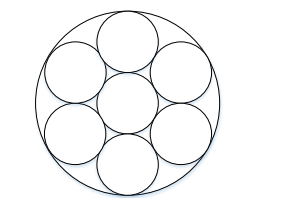
\includegraphics[width= 0.4\columnwidth]{figs/circle.png}
    \caption*{Q.no 7}
    \label{fig:q7}
\end{figure}
The length of the container is equal to the length of the chalk-sticks. The ratio of the occupied space to the empty space of the container is \rule{3cm}{0.15mm}. \hfill{\brak{\text{GATE MA 2024}}}
\begin{enumerate}
    \begin{multicols}{4}
    \item $5/2$
    \item $7/2$
    \item $9/2$
    \item $3$
    \end{multicols}
\end{enumerate}

% Question 8
\item The plot below shows the relationship between the mortality risk of cardiovascular disease and the number of steps a person walks per day. Based on the data, which one of the following options is true?
\begin{figure}[h!]
    \centering
    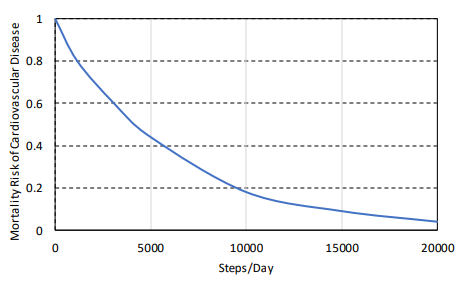
\includegraphics[width=0.6\columnwidth]{figs/graph.png}
    \caption*{Q.no 8}
    \label{fig:q8}
\end{figure}
\hfill{\brak{\text{GATE MA 2024}}}
\begin{enumerate}
    \item The risk reduction on increasing the steps/day from $0$ to $10000$ is less than the risk reduction on increasing the steps/day from $10000$ to $20000$.
    \item The risk reduction on increasing the steps/day from $0$ to $5000$ is less than the risk reduction on increasing the steps/day from $15000$ to $20000$.
    \item For any $5000$ increment in steps/day the largest risk reduction occurs on going from $0$ to $5000$.
    \item For any $5000$ increment in steps/day the largest risk reduction occurs on going from $15000$ to $20000$.
\end{enumerate}

% Question 9
\item Five cubes of identical size and another smaller cube are assembled as shown in Figure A. If viewed from direction X, the planar image of the assembly appears as Figure B.If viewed from direction Y, the planar image of the assembly Figure A will appear as 
\begin{figure}[h!]
    \centering
    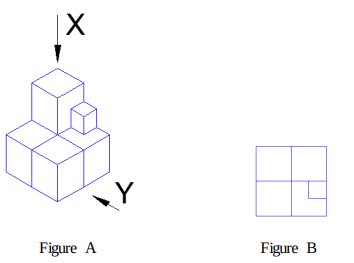
\includegraphics[width=0.3\columnwidth]{figs/question.png}
    \caption*{Q.no 9}
    \label{fig:q9}
\end{figure}
\hfill{\brak{\text{GATE MA 2024}}}
\begin{enumerate}
\begin{multicols}{2}
    \begin{figure}[H]
   \item  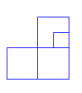
\includegraphics[width=0.2\columnwidth]{figs/que 1.png}
   \item 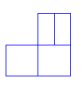
\includegraphics[width=0.2\columnwidth]{figs/que 2.png}
    \item 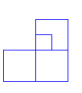
\includegraphics[width=0.2\columnwidth]{figs/que 3.png}
    \item 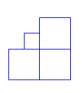
\includegraphics[width=0.2\columnwidth]{figs/que 4.png}
    \caption*{Q.no 9 options}
    \label{fig:q9options}
    \end{figure}
    \end{multicols}
\end{enumerate}
% Question 10
\item Visualize a cube that is held with one of the four body diagonals aligned to the vertical axis. Rotate the cube about this axis such that its view remains unchanged. The magnitude of the minimum angle of rotation is \rule{3cm}{0.15mm}. \hfill{\brak{\text{GATE MA 2024}}}
\begin{enumerate}
    \begin{multicols}{4}
    \item $120\degree$
    \item $60\degree$
    \item $90\degree$
    \item $180\degree$
    \end{multicols}
\end{enumerate}

% Question 11
\item Consider the following condition on a function $f \colon \mathbb{C} \to \mathbb{C}$
\[ \abs{f\brak{z}} = 1 \text{ for all } z \in \mathbb{C} \text{ such that } \text{Im}\brak{z} = 0. \quad \brak{P} \]
Which one of the following is correct? \hfill{\brak{\text{GATE MA 2024}}}
\begin{enumerate}
    \item There is a non-constant analytic polynomial $f$ satisfying \brak{P}
    \item Every entire function $f$ satisfying \brak{P} is a constant function
    \item Every entire function $f$ satisfying \brak{P} has no zeroes in $\mathbb{C}$
    \item There is an entire function $f$ satisfying \brak{P} with infinitely many zeroes in $\mathbb{C}$
\end{enumerate}

% Question 12
\item Let $C$ be the ellipse $\{z \in \mathbb{C} \colon \abs{z - 2} + \abs{z + 2} = 8\}$ traversed counter-clockwise. The value of the contour integral
\[ \int_C \frac{z^2 dz}{z^2 - 2z + 2} \]
is equal to \hfill{\brak{\text{GATE MA 2024}}}
\begin{enumerate}
    \begin{multicols}{4}
    \item $0$
    \item $2\pi i$
    \item $4\pi i$
    \item $-\pi i$
    \end{multicols}
\end{enumerate}

% Question 13
\item Let $X$ be a topological space and $A \subseteq X$. Given a subset $S$ of $X$, let $\text{int}\brak{S}$, $\partial S$, and $\bar{S}$ denote the interior, boundary, and closure, respectively, of the set $S$. Which one of the following is NOT necessarily true? \hfill{\brak{\text{GATE MA 2024}}}
\begin{enumerate}
    \item $\text{int}\brak{X \setminus A} \subseteq X \setminus \bar{A}$
    \item $\bar{A} \subseteq \overline{\text{int}\brak{A}}$
    \item $\partial A \subseteq \partial \brak{\text{int}\brak{A}}$
    \item $\partial \bar{A} \subseteq \partial A$
\end{enumerate}

% Question 14
\item Consider the following limit
\[ \lim_{\varepsilon \to 0} \frac{1}{\varepsilon} \int_0^\infty e^{-x/\varepsilon} \brak{\cos\brak{3x} + x^2 + \sqrt{x} + 4} dx. \]
Which one of the following is correct? \hfill{\brak{\text{GATE MA 2024}}}
\begin{enumerate}
    \item The limit does not exist
    \item The limit exists and is equal to $0$
    \item The limit exists and is equal to $3$
    \item The limit exists and is equal to $\pi$
\end{enumerate}

% Question 15
\item Let $\mathbb{R}[X^2, X^3]$ be the subring of $\mathbb{R}[X]$ generated by $X^2$ and $X^3$. Consider the following statements.
\begin{enumerate}
    \item[I.] The ring $\mathbb{R}[X^2, X^3]$ is a unique factorization domain.
    \item[II.] The ring $\mathbb{R}[X^2, X^3]$ is a principal ideal domain.
\end{enumerate}
Which one of the following is correct? \hfill{\brak{\text{GATE MA 2024}}}
\begin{enumerate}
    \item Both I and II are TRUE
    \item I is TRUE and II is FALSE
    \item I is FALSE and II is TRUE
    \item Both I and II are FALSE
\end{enumerate}

% Question 16
\item Given a prime number $p$, let $n_p\brak{G}$ denote the number of $p$-Sylow subgroups of a finite group $G$. Which one of the following is TRUE for every group $G$ of order $2024$? \hfill{\brak{\text{GATE MA 2024}}}
\begin{enumerate}
    \item $n_{11}\brak{G} = 1$ and $n_{23}\brak{G} = 11$
    \item $n_{11}\brak{G} \in \{1, 23\}$ and $n_{23}\brak{G} = 1$
    \item $n_{11}\brak{G} = 23$ and $n_{23}\brak{G} \in \{1, 88\}$
    \item $n_{11}\brak{G} = 23$ and $n_{23}\brak{G} = 11$
\end{enumerate}

% Question 17
\item Consider the following statements.
\begin{enumerate}
    \item[I.] Every compact Hausdorff space is normal.
    \item[II.] Every metric space is normal.
\end{enumerate}
Which one of the following is correct? \hfill{\brak{\text{GATE MA 2024}}}
\begin{enumerate}
    \item Both I and II are TRUE
    \item I is TRUE and II is FALSE
    \item I is FALSE and II is TRUE
    \item Both I and II are FALSE
\end{enumerate}

% Question 18
\item Consider the topology on $\mathbb{Z}$ with basis $\{S\brak{a, b} \colon a, b \in \mathbb{Z} \text{ and } a \neq 0\}$, where $S\brak{a, b} = \{an + b \colon n \in \mathbb{Z}\}$. Consider the following statements.
\begin{enumerate}
    \item[I.] $S\brak{a, b}$ is both open and closed for each $a, b \in \mathbb{Z}$ with $a \neq 0$.
    \item[II.] The only connected set containing $x \in \mathbb{Z}$ is $\{x\}$.
\end{enumerate}
Which one of the following is correct? \hfill{\brak{\text{GATE MA 2024}}}
\begin{enumerate}
    \item Both I and II are TRUE
    \item I is TRUE and II is FALSE
    \item I is FALSE and II is TRUE
    \item Both I and II are FALSE
\end{enumerate}

% Question 19
\item Let $A = \myvec{0 & 2 \\ 2 & 0}$ and $T \colon M_2\brak{\mathbb{C}} \to M_2\brak{\mathbb{C}}$ be the linear transformation given by $T\brak{B} = AB$. The characteristic polynomial of $T$ is \hfill{\brak{\text{GATE MA 2024}}}
\begin{enumerate}
    \begin{multicols}{2}
    \item $X^4 - 8X^2 + 16$
    \item $X^2 - 4$
    \item $X^2 - 2$
    \item $X^4 - 16$
    \end{multicols}
\end{enumerate}

% Question 20
\item Let $A \in M_n\brak{\mathbb{C}}$ be a normal matrix. Consider the following statements.
\begin{enumerate}
    \item[I.] If all the eigenvalues of $A$ are real, then $A$ is Hermitian.
    \item[II.] If all the eigenvalues of $A$ have absolute value $1$, then $A$ is unitary.
\end{enumerate}
Which one of the following is correct? \hfill{\brak{\text{GATE MA 2024}}}
\begin{enumerate}
    \item Both I and II are TRUE
    \item I is TRUE and II is FALSE
    \item I is FALSE and II is TRUE
    \item Both I and II are FALSE
\end{enumerate}

% Question 21
\item Let $A = \myvec{2 & -1 & 1 \\ 1 & 2 & -1 \\ -1 & 1 & 2}$ and $b$ be a $3 \times 1$ real column vector. Consider the statements.
\begin{enumerate}
    \item[I.] The Jacobi iteration method for the system $\brak{A + \varepsilon I_3}x = b$ converges for any initial approximation and $\varepsilon > 0$.
    \item[II.] The Gauss-Seidel iteration method for the system $\brak{A + \varepsilon I_3}x = b$ converges for any initial approximation and $\varepsilon > 0$.
\end{enumerate}
Which one of the following is correct? \hfill{\brak{\text{GATE MA 2024}}}
\begin{enumerate}
    \item Both I and II are TRUE
    \item I is TRUE and II is FALSE
    \item I is FALSE and II is TRUE
    \item Both I and II are FALSE
\end{enumerate}

% Question 22
\item For the initial value problem $y' = f\brak{x, y}$, $y\brak{x_0} = y_0$, generate approximations $y_n$ to $y\brak{x_n}$, $x_n = x_0 + nh$, for a fixed $h > 0$ and $n = 1, 2, 3, \dots$, using the recursion formula
\[ y_n = y_{n-1} + ak_1 + bk_2, \text{ where} \]
\[ k_1 = hf\brak{x_{n-1}, y_{n-1}} \text{ and } k_2 = hf\brak{x_{n-1} + \alpha h, y_{n-1} + \beta k_1}. \]
Which one of the following choices of $a, b, \alpha, \beta$ for the above recursion formula gives the Runge-Kutta method of order $2$? \hfill{\brak{\text{GATE MA 2024}}}
\begin{enumerate}
    \item $a = 1, b = 1, \alpha = 0.5, \beta = 0.5$
    \item $a = 0.5, b = 0.5, \alpha = 2, \beta = 2$
    \item $a = 0.25, b = 0.75, \alpha = 2/3, \beta = 2/3$
    \item $a = 0.5, b = 0.5, \alpha = 1, \beta = 2$
\end{enumerate}

% Question 23
\item Let $u = u\brak{x, t}$ be the solution of
\begin{align*}
    \frac{\partial u}{\partial t} - 4\frac{\partial^2 u}{\partial x^2} &= 0, \quad 0 < x < 1, t > 0, \\
    u\brak{0, t} = u\brak{1, t} &= 0, \quad t \ge 0, \\
    u\brak{x, 0} &= \sin\brak{\pi x}, \quad 0 \le x \le 1.
\end{align*}
Define $g\brak{t} = \int_0^1 \brak{u\brak{x, t}}^2 dx$, for $t > 0$. Which one of the following is correct? \hfill{\brak{\text{GATE MA 2024}}}
\begin{enumerate}
    \item $g$ is decreasing on $\brak{0, \infty}$ and $\lim_{t\to\infty} g\brak{t} = 0$
    \item $g$ is decreasing on $\brak{0, \infty}$ and $\lim_{t\to\infty} g\brak{t} = 1/4$
    \item $g$ is increasing on $\brak{0, \infty}$ and $\lim_{t\to\infty} g\brak{t}$ does not exist
    \item $g$ is increasing on $\brak{0, \infty}$ and $\lim_{t\to\infty} g\brak{t} = 3$
\end{enumerate}

% Question 24
\item If $y_1$ and $y_2$ are two different solutions of the ordinary differential equation $y' + \sin\brak{e^x}y = \cos\brak{e^{x+1}}$, $0 \le x \le 1$, then which one of the following is its general solution on $[0, 1]$? \hfill{\brak{\text{GATE MA 2024}}}
\begin{enumerate}
    \item $c_1 y_1 + c_2 y_2, c_1, c_2 \in \mathbb{R}$
    \item $y_1 + c\brak{y_1 - y_2}, c \in \mathbb{R}$
    \item $cy_1 + \brak{y_1 - y_2}, c \in \mathbb{R}$
    \item $c_1\brak{y_1 + y_2} + c_2\brak{y_1 - y_2}, c_1, c_2 \in \mathbb{R}$
\end{enumerate}

% Question 25
\item Consider the following Linear Programming Problem P
\begin{align*}
    \text{minimize } & 5x_1 + 2x_2 \\
    \text{subject to } & 2x_1 + x_2 \le 2, \\
    & x_1 + x_2 \ge 1, \\
    & x_1, x_2 \ge 0.
\end{align*}
The optimal value of the problem P is equal to \hfill{\brak{\text{GATE MA 2024}}}
\begin{enumerate}
    \begin{multicols}{4}
    \item $5$
    \item $0$
    \item $4$
    \item $2$
    \end{multicols}
\end{enumerate}

% Question 26
\item Let $p = \brak{1, 1/2, 1/3, 1/4} \in \mathbb{R}^4$ and $f \colon \mathbb{R}^4 \to \mathbb{R}$ be a differentiable function such that $f\brak{p} = 6$ and $f\brak{\lambda x} = \lambda^3 f\brak{x}$, for every $\lambda \in \brak{0, \infty}$ and $x \in \mathbb{R}^4$. The value of
\[ 12\frac{\partial f}{\partial x_1}\brak{p} + 6\frac{\partial f}{\partial x_2}\brak{p} + 4\frac{\partial f}{\partial x_3}\brak{p} + 3\frac{\partial f}{\partial x_4}\brak{p} \]
is equal to \rule{3cm}{0.15mm} \brak{\text{answer in integer}}. \hfill{\brak{\text{GATE MA 2024}}}

% Question 27
\item The number of non-isomorphic finite groups with exactly $3$ conjugacy classes is equal to \rule{3cm}{0.15mm} \brak{\text{answer in integer}}. \hfill{\brak{\text{GATE MA 2024}}}

% Question 28
\item Let $f\brak{x, y} = \brak{x^2 - y^2, 2xy}$, where $x > 0, y > 0$. Let $g$ be the inverse of $f$ in a neighborhood of $f\brak{2, 1}$. Then the determinant of the Jacobian matrix of $g$ at $f\brak{2, 1}$ is equal to \rule{3cm}{0.15mm} \brak{\text{round off to TWO decimal places}}. \hfill{\brak{\text{GATE MA 2024}}}

% Question 29
\item Let $\mathbb{F}_3$ be the field with exactly $3$ elements. The number of elements in $GL_2\brak{\mathbb{F}_3}$ is equal to \rule{3cm}{0.15mm} \brak{\text{answer in integer}}. \hfill{\brak{\text{GATE MA 2024}}}

% Question 30
\item Given a real subspace $W$ of $\mathbb{R}^4$, let $W^\perp$ denote its orthogonal complement with respect to the standard inner product on $\mathbb{R}^4$. Let $W_1 = \text{Span}\{(1, 0, 0, -1)\}$ and $W_2 = \text{Span}\{(2, 1, 0, -1)\}$ be real subspaces of $\mathbb{R}^4$. The dimension of $W_1^\perp \cap W_2^\perp$ over $\mathbb{R}$ is equal to \rule{3cm}{0.15mm} \brak{\text{answer in integer}}. \hfill{\brak{\text{GATE MA 2024}}}

% Question 31
\item The number of group homomorphisms from $\mathbb{Z}/4\mathbb{Z}$ to $S_4$ is equal to \rule{3cm}{0.15mm} \brak{\text{answer in integer}}. \hfill{\brak{\text{GATE MA 2024}}}

% Question 32
\item Let $a \in \mathbb{R}$ and $h$ be a positive real number. For any twice-differentiable function $f \colon \mathbb{R} \to \mathbb{R}$, let $P_f\brak{x}$ be the interpolating polynomial of degree at most two that interpolates $f$ at the points $a-h, a, a+h$. Define $d$ to be the largest integer such that any polynomial $g$ of degree $d$ satisfies $g''\brak{a} = P''_g\brak{a}$. The value of $d$ is equal to \rule{3cm}{0.15mm} \brak{\text{answer in integer}}. \hfill{\brak{\text{GATE MA 2024}}}

% Question 33
\item Let $P_f\brak{x}$ be the interpolating polynomial of degree at most two that interpolates the function $f\brak{x} = x^2\abs{x}$ at the points $x = -1, 0, 1$. Then $\sup_{x \in [-1, 1]} \abs{f\brak{x} - P_f\brak{x}} = $ \rule{3cm}{0.15mm} \brak{\text{round off to TWO decimal places}}. \hfill{\brak{\text{GATE MA 2024}}}

% Question 34
\item The maximum of the function $f\brak{x, y, z} = xyz$ subject to the constraints $xy + yz + zx = 12$, $x > 0, y > 0, z > 0$, is equal to \rule{3cm}{0.15mm} \brak{\text{round off to TWO decimal places}}. \hfill{\brak{\text{GATE MA 2024}}}

% Question 35
\item If the outward flux of $F\brak{x, y, z} = \brak{x^3, y^3, z^3}$ through the unit sphere $x^2 + y^2 + z^2 = 1$ is $\alpha\pi$, then $\alpha$ is equal to \rule{3cm}{0.15mm} \brak{\text{round off to TWO decimal places}}. \hfill{\brak{\text{GATE MA 2024}}}

% Question 36
\item Let $H = \{z \in \mathbb{C} \colon \text{Im}\brak{z} > 0\}$ and $D = \{z \in \mathbb{C} \colon \abs{z} < 1\}$. Then
\[ \sup \{ \abs{f'\brak{0}} \colon f \text{ is an analytic function from } D \text{ to } H \text{ and } f\brak{0} = i/2 \} \]
is equal to \hfill{\brak{\text{GATE MA 2024}}}
\begin{enumerate}
    \begin{multicols}{4}
    \item $\frac{1}{4}$
    \item $\frac{1}{2}$
    \item $1$
    \item $100$
    \end{multicols}
\end{enumerate}

% Question 37
\item Let $S_1 = \{z \in \mathbb{C} \colon \abs{z} = 1\}$. For which one of the following functions $f$ does there exist a sequence of polynomials in $z$ that uniformly converges to $f$ on $S_1$? \hfill{\brak{\text{GATE MA 2024}}}
\begin{enumerate}
    \item $f\brak{z} = \bar{z}$
    \item $f\brak{z} = \text{Re}\brak{z}$
    \item $f\brak{z} = e^{\bar{z}}$
    \item $f\brak{z} = \abs{z+1}^2$
\end{enumerate}

% Question 38
\item Let $f \colon [0, 1] \to \mathbb{R}$ be a function. Which one of the following is a sufficient condition for $f$ to be Lebesgue measurable? \hfill{\brak{\text{GATE MA 2024}}}
\begin{enumerate}
    \item $\abs{f}$ is a Lebesgue measurable function
    \item There exist continuous functions $g, h \colon [0, 1] \to \mathbb{R}$ such that $g \le f \le h$ on $[0, 1]$
    \item $f$ is continuous almost everywhere on $[0, 1]$
    \item For each $c \in \mathbb{R}$, the set $\{x \in [0, 1] \colon f\brak{x} = c\}$ is Lebesgue measurable
\end{enumerate}

% Question 39
\item Let $g \colon M_2\brak{\mathbb{R}} \to \mathbb{R}$ be given by $g\brak{A} = \text{Trace}\brak{A^2}$. Let $0$ be the $2 \times 2$ zero matrix. The space $M_2\brak{\mathbb{R}}$ may be identified with $\mathbb{R}^4$ in the usual manner. Which one of the following is correct? \hfill{\brak{\text{GATE MA 2024}}}
\begin{enumerate}
    \item $0$ is a point of local minimum of $g$
    \item $0$ is a point of local maximum of $g$
    \item $0$ is a saddle point of $g$
    \item $0$ is not a critical point of $g$
\end{enumerate}

% Question 40
\item Consider the following statements.
\begin{enumerate}
    \item[I.] There exists a proper subgroup $G$ of $\brak{\mathbb{Q}, +}$ such that $\mathbb{Q}/G$ is a finite group.
    \item[II.] There exists a subgroup $G$ of $\brak{\mathbb{Q}, +}$ such that $\mathbb{Q}/G$ is isomorphic to $\brak{\mathbb{Z}, +}$.
\end{enumerate}
Which one of the following is correct? \hfill{\brak{\text{GATE MA 2024}}}
\begin{enumerate}
    \item Both I and II are TRUE
    \item I is TRUE and II is FALSE
    \item I is FALSE and II is TRUE
    \item Both I and II are FALSE
\end{enumerate}

% Question 41
\item Let $X$ be the space $\mathbb{R}/\mathbb{Z}$ with the quotient topology induced from the usual topology on $\mathbb{R}$. Consider the following statements.
\begin{enumerate}
    \item[I.] $X$ is compact.
    \item[II.] $X \setminus \{x\}$ is connected for any $x \in X$.
\end{enumerate}
Which one of the following is correct? \hfill{\brak{\text{GATE MA 2024}}}
\begin{enumerate}
    \item Both I and II are TRUE
    \item I is TRUE and II is FALSE
    \item I is FALSE and II is TRUE
    \item Both I and II are FALSE
\end{enumerate}

% Question 42
\item Let $\langle \cdot, \cdot \rangle$ denote the standard inner product on $\mathbb{R}^7$. Let $\Sigma = \{v_1, \dots, v_5\} \subseteq \mathbb{R}^7$ be a set of unit vectors such that $\langle v_i, v_j \rangle$ is a non-positive integer for all $1 \le i \neq j \le 5$. Define $N\brak{\Sigma}$ to be the number of pairs $\brak{r, s}$, $1 \le r, s \le 5$, such that $\langle v_r, v_s \rangle \neq 0$. The maximum possible value of $N\brak{\Sigma}$ is equal to \hfill{\brak{\text{GATE MA 2024}}}
\begin{enumerate}
    \begin{multicols}{4}
    \item $9$
    \item $10$
    \item $14$
    \item $5$
    \end{multicols}
\end{enumerate}

% Question 43
\item Let $f\brak{x} = \abs{x} + \abs{x-1} + \abs{x-2}$, $x \in [-1, 2]$. Which one of the following numerical integration rules gives the exact value of the integral $\int_{-1}^2 f\brak{x} dx$? \hfill{\brak{\text{GATE MA 2024}}}
\begin{enumerate}
    \item The Simpson's rule
    \item The trapezoidal rule
    \item The composite Simpson's rule by dividing $[-1, 2]$ into $4$ equal subintervals
    \item The composite trapezoidal rule by dividing $[-1, 2]$ into $3$ equal subintervals
\end{enumerate}

% Question 44
\item Consider the initial value problem \brak{IVP}
\[ y' = e^{-y^2} + 1, \quad y\brak{0} = 0. \]
\begin{enumerate}
    \item[I.] IVP has a unique solution on $\mathbb{R}$.
    \item[II.] Every solution of IVP is bounded on its maximal interval of existence.
\end{enumerate}
Which one of the following is correct? \hfill{\brak{\text{GATE MA 2024}}}
\begin{enumerate}
    \item Both I and II are TRUE
    \item I is TRUE and II is FALSE
    \item I is FALSE and II is TRUE
    \item Both I and II are FALSE
\end{enumerate}

% Question 45
\item Let $A$ be a $2 \times 2$ non-diagonalizable real matrix with a real eigenvalue $\lambda$ and $v$ be an eigenvector of $A$ corresponding to $\lambda$. Which one of the following is the general solution of the system $y' = Ay$ of first-order linear differential equations? \hfill{\brak{\text{GATE MA 2024}}}
\begin{enumerate}
    \item $c_1 e^{\lambda t} v + c_2 t e^{\lambda t} v$, where $c_1, c_2 \in \mathbb{R}$
    \item $c_1 e^{\lambda t} v + c_2 t^2 e^{\lambda t} v$, where $c_1, c_2 \in \mathbb{R}$
    \item $c_1 e^{\lambda t} v + c_2 e^{\lambda t} \brak{tv + u}$, where $c_1, c_2 \in \mathbb{R}$ and $u$ is a $2 \times 1$ real column vector such that $\brak{A - \lambda I_2}u = v$
    \item $c_1 e^{\lambda t} v + c_2 t e^{\lambda t} \brak{v + u}$, where $c_1, c_2 \in \mathbb{R}$ and $u$ is a $2 \times 1$ real column vector such that $\brak{A - \lambda I_2}u = v$
\end{enumerate}

% Question 46
\item Let $D = \{(x, y) \in \mathbb{R}^2 \colon x > 0 \text{ and } y > 0\}$. If the following second-order linear partial differential equation
\[ y^2 \frac{\partial^2 u}{\partial x^2} - x^2 \frac{\partial^2 u}{\partial y^2} + y \frac{\partial u}{\partial y} = 0 \text{ on } D \]
is transformed to
\[ \frac{\partial^2 u}{\partial \eta^2} - \frac{\partial^2 u}{\partial \xi^2} + \brak{\frac{\partial u}{\partial \eta} + \frac{\partial u}{\partial \xi}} \frac{1}{2\eta} + \brak{a\frac{\partial u}{\partial \eta} + b\frac{\partial u}{\partial \xi}} \frac{1}{2\xi} = 0 \text{ on } D \]
for some $a, b \in \mathbb{R}$, via the co-ordinate transform $\eta = x^2/2$ and $\xi = y^2/2$, then which one of the following is correct? \hfill{\brak{\text{GATE MA 2024}}}
\begin{enumerate}
    \item $a = 2, b = 0$
    \item $a = 0, b = -1$
    \item $a = 1, b = -1$
    \item $a = 1, b = 0$
\end{enumerate}

% Question 47
\item Let $\ell^p = \left\{ x = \brak{x_n}_{n\ge 1} \colon x_n \in \mathbb{R}, \|x\|_p = \brak{\sum_{n=1}^\infty \abs{x_n}^p}^{1/p} < \infty \right\}$ for $p=1, 2$. Let $C_{00} = \{\brak{x_n}_{n\ge 1} \colon x_n = 0 \text{ for all but finitely many } n \ge 1\}$. For $x = \brak{x_n}_{n\ge 1} \in C_{00}$, define $f\brak{x} = \sum_{n=1}^\infty \frac{x_n}{\sqrt{n}}$. Consider the following statements.
\begin{enumerate}
    \item[I.] There exists a continuous linear functional $F$ on $\brak{\ell^1, \|\cdot\|_1}$ such that $F=f$ on $C_{00}$.
    \item[II.] There exists a continuous linear functional $G$ on $\brak{\ell^2, \|\cdot\|_2}$ such that $G=f$ on $C_{00}$.
\end{enumerate}
Which one of the following is correct? \hfill{\brak{\text{GATE MA 2024}}}
\begin{enumerate}
    \item Both I and II are TRUE
    \item I is TRUE and II is FALSE
    \item I is FALSE and II is TRUE
    \item Both I and II are FALSE
\end{enumerate}

% Question 48
\item Let $\ell^2_{\mathbb{Z}} = \left\{ \brak{x_j}_{j \in \mathbb{Z}} \colon x_j \in \mathbb{R} \text{ and } \sum_{j=-\infty}^\infty x_j^2 < \infty \right\}$ endowed with the inner product $\langle x, y \rangle = \sum_{j=-\infty}^\infty x_j y_j$, $x = \brak{x_j}_{j \in \mathbb{Z}}, y = \brak{y_j}_{j \in \mathbb{Z}} \in \ell^2_{\mathbb{Z}}$. Let $T \colon \ell^2_{\mathbb{Z}} \to \ell^2_{\mathbb{Z}}$ be given by $T\brak{\brak{x_j}_{j \in \mathbb{Z}}} = \brak{y_j}_{j \in \mathbb{Z}}$, where $y_j = \frac{x_j + x_{-j}}{2}, j \in \mathbb{Z}$. Which of the following is/are correct? \hfill{\brak{\text{GATE MA 2024}}}
\begin{enumerate}
    \item $T$ is a compact operator
    \item The operator norm of $T$ is $1$
    \item $T$ is a self-adjoint operator
    \item Range$\brak{T}$ is closed
\end{enumerate}

% Question 49
\item Let $X$ be the normed space $\brak{\mathbb{R}^2, \|\cdot\|}$, where $\|\brak{x, y}\| = \abs{x} + \abs{y}$, $\brak{x, y} \in \mathbb{R}^2$. Let $S = \{\brak{x, 0} \colon x \in \mathbb{R}\}$ and $f \colon S \to \mathbb{R}$ be given by $f\brak{\brak{x, 0}} = 2x$ for all $x \in \mathbb{R}$. Recall that a Hahn-Banach extension of $f$ to $X$ is a continuous linear functional $F$ on $X$ such that $F|_S = f$ and $\|F\| = \|f\|$, where $\|F\|$ and $\|f\|$ are the norms of $F$ and $f$ on $X$ and $S$, respectively. Which of the following is/are true? \hfill{\brak{\text{GATE MA 2024}}}
\begin{enumerate}
    \item $F\brak{x, y} = 2x + 3y$ is a Hahn-Banach extension of $f$ to $X$
    \item $F\brak{x, y} = 2x + y$ is a Hahn-Banach extension of $f$ to $X$
    \item $f$ admits infinitely many Hahn-Banach extensions to $X$
    \item $f$ admits exactly two distinct Hahn-Banach extensions to $X$
\end{enumerate}

% Question 50
\item Let $\{[a, b) \colon a, b \in \mathbb{R}, a < b\}$ be a basis for a topology $\tau$ on $\mathbb{R}$. Which of the following is/are correct? \hfill{\brak{\text{GATE MA 2024}}}
\begin{enumerate}
    \item Every $\brak{a, b}$ with $a < b$ is an open set in $\brak{\mathbb{R}, \tau}$
    \item Every $[a, b]$ with $a < b$ is a compact set in $\brak{\mathbb{R}, \tau}$
    \item $\brak{\mathbb{R}, \tau}$ is a first-countable space
    \item $\brak{\mathbb{R}, \tau}$ is a second-countable space
\end{enumerate}

% Question 51
\item Let $T, S \colon \mathbb{R}^4 \to \mathbb{R}^4$ be two non-zero, non-identity $\mathbb{R}$-linear transformations. Assume $T^2 = T$. Which of the following is/are TRUE? \hfill{\brak{\text{GATE MA 2024}}}
\begin{enumerate}
    \item $T$ is necessarily invertible
    \item $T$ and $S$ are similar if $S^2 = S$ and Rank$\brak{T}$ = Rank$\brak{S}$
    \item $T$ and $S$ are similar if $S$ has only $0$ and $1$ as eigenvalues
    \item $T$ is necessarily diagonalizable
\end{enumerate}

% Question 52
\item Let $p_1 < p_2$ be the two fixed points of the function $g\brak{x} = e^x - 2$, where $x \in \mathbb{R}$. For $x_0 \in \mathbb{R}$, let the sequence $\brak{x_n}_{n \ge 1}$ be generated by the fixed point iteration $x_n = g\brak{x_{n-1}}, n \ge 1$. Which one of the following is/are correct? \hfill{\brak{\text{GATE MA 2024}}}
\begin{enumerate}
    \item $\brak{x_n}_{n\ge 0}$ converges to $p_1$ for any $x_0 \in \brak{p_1, p_2}$
    \item $\brak{x_n}_{n\ge 0}$ converges to $p_2$ for any $x_0 \in \brak{p_1, p_2}$
    \item $\brak{x_n}_{n\ge 0}$ converges to $p_2$ for any $x_0 > p_2$
    \item $\brak{x_n}_{n\ge 0}$ converges to $p_1$ for any $x_0 < p_1$
\end{enumerate}

% Question 53
\item Which of the following is/are eigenvalue\brak{s} of the Sturm-Liouville problem
\begin{align*}
    y'' + \lambda y &= 0, \quad 0 \le x \le \pi, \\
    y\brak{0} &= y'\brak{0}, \\
    y\brak{\pi} &= y'\brak{\pi}?
\end{align*}
\hfill{\brak{\text{GATE MA 2024}}}
\begin{enumerate}
    \item $\lambda = 1$
    \item $\lambda = 2$
    \item $\lambda = 3$
    \item $\lambda = 4$
\end{enumerate}

% Question 54
\item Let $f \colon \mathbb{R}^2 \to \mathbb{R}$ be a function such that
\[ f\brak{x, y} = \begin{cases} \frac{1 - \cos\brak{x^2y^2}}{\sqrt{x^2+y^2}}, & \text{if } y \neq 0, x \in \mathbb{R}, \\ 0, & \text{otherwise.} \end{cases} \]
Which of the following is/are correct? \hfill{\brak{\text{GATE MA 2024}}}
\begin{enumerate}
    \item $f$ is continuous at $\brak{0, 0}$, but not differentiable at $\brak{0, 0}$
    \item $f$ is differentiable at $\brak{0, 0}$
    \item All the directional derivatives of $f$ at $\brak{0, 0}$ exist and they are equal to zero
    \item Both the partial derivatives of $f$ at $\brak{0, 0}$ exist and they are equal to zero
\end{enumerate}

% Question 55
\item For an integer $n$, let $f_n\brak{x} = xe^{-nx}$, where $x \in [0, 1]$. Let $S := \{f_n \colon n \ge 1\}$. Consider the metric space $\brak{C\brak{[0, 1]}, d}$, where $d\brak{f, g} = \sup_{x \in [0, 1]} \{\abs{f\brak{x} - g\brak{x}}\}$, $f, g \in C\brak{[0, 1]}$. Which of the following statement\brak{s} is/are true? \hfill{\brak{\text{GATE MA 2024}}}
\begin{enumerate}
    \item $S$ is an equi-continuous family of continuous functions
    \item $S$ is closed in $\brak{C\brak{[0, 1]}, d}$
    \item $S$ is bounded in $\brak{C\brak{[0, 1]}, d}$
    \item $S$ is compact in $\brak{C\brak{[0, 1]}, d}$
\end{enumerate}

% Question 56
\item Let $T \colon \mathbb{R}^4 \to \mathbb{R}^4$ be an $\mathbb{R}$-linear transformation such that $1$ and $2$ are the only eigenvalues of $T$. Suppose the dimensions of Kernel$\brak{T - I_4}$ and Range$\brak{T - 2I_4}$ are $1$ and $2$, respectively. Which of the following is/are possible \brak{\text{upper triangular}} Jordan canonical form\brak{s} of $T$? \hfill{\brak{\text{GATE MA 2024}}}
\begin{enumerate}
    \item $\myvec{1 & 0 & 0 & 0 \\ 0 & 2 & 0 & 0 \\ 0 & 0 & 2 & 1 \\ 0 & 0 & 0 & 2}$
    \item $\myvec{1 & 0 & 0 & 0 \\ 0 & 2 & 1 & 0 \\ 0 & 0 & 2 & 1 \\ 0 & 0 & 0 & 2}$
    \item $\myvec{1 & 1 & 0 & 0 \\ 0 & 1 & 0 & 0 \\ 0 & 0 & 2 & 1 \\ 0 & 0 & 0 & 2}$
    \item $\myvec{1 & 1 & 0 & 0 \\ 0 & 1 & 0 & 0 \\ 0 & 0 & 2 & 0 \\ 0 & 0 & 0 & 2}$
\end{enumerate}

% Question 57
\item Let $L^2\brak{[-1, 1]}$ denote the space of all real-valued Lebesgue square-integrable functions on $[-1, 1]$, with the usual norm $\|\cdot\|$. Let $P_1$ be the subspace of $L^2\brak{[-1, 1]}$ consisting of all the polynomials of degree at most $1$. Let $f \in L^2\brak{[-1, 1]}$ be such that $\|f\|^2 = 18/5$, $\int_{-1}^1 f\brak{x} dx = 2$, and $\int_{-1}^1 xf\brak{x} dx = 0$. Then $\inf_{g \in P_1} \|f-g\|^2 =$ \rule{3cm}{0.15mm} \brak{\text{round off to TWO decimal places}}. \hfill{\brak{\text{GATE MA 2024}}}

% Question 58
\item The maximum value of $f\brak{x, y, z} = 10x + 6y - 8z$ subject to the constraints
\begin{align*}
    5x - 2y + 6z &\le 20, \\
    10x + 4y - 6z &\le 30, \\
    x, y, z &\ge 0,
\end{align*}
is equal to \rule{3cm}{0.15mm} \brak{\text{round off to TWO decimal places}}. \hfill{\brak{\text{GATE MA 2024}}}

% Question 59
\item Let $K \subseteq \mathbb{C}$ be the field extension of $\mathbb{Q}$ obtained by adjoining all the roots of the polynomial equation $\brak{X^2 - 2}\brak{X^2 - 3} = 0$. The number of distinct fields $F$ such that $\mathbb{Q} \subseteq F \subseteq K$ is equal to \rule{3cm}{0.15mm} \brak{\text{answer in integer}}. \hfill{\brak{\text{GATE MA 2024}}}

% Question 60
\item Let $H$ be the subset of $S_3$ consisting of all $\sigma \in S_3$ such that Trace$\brak{A_1 A_2 A_3} = \text{Trace}\brak{A_{\sigma\brak{1}} A_{\sigma\brak{2}} A_{\sigma\brak{3}}}$, for all $A_1, A_2, A_3 \in M_2\brak{\mathbb{C}}$. The number of elements in $H$ is equal to \rule{3cm}{0.15mm} \brak{\text{answer in integer}}. \hfill{\brak{\text{GATE MA 2024}}}

% Question 61
\item Let $r \colon [0, 1] \to \mathbb{R}^2$ be a continuously differentiable path from $\brak{0, 2}$ to $\brak{3, 0}$ and let $F \colon \mathbb{R}^2 \to \mathbb{R}^2$ be defined by $F\brak{x, y} = \brak{1 - 2y, 1 - 2x}$. The line integral of $F$ along $r$
\[ \int_r F \cdot dr \]
is equal to \rule{3cm}{0.15mm} \brak{\text{round off to TWO decimal places}}. \hfill{\brak{\text{GATE MA 2024}}}

% Question 62
\item Let $u = u\brak{x, t}$ be the solution of the initial value problem
\begin{align*}
    \frac{\partial^2 u}{\partial t^2} - \frac{\partial^2 u}{\partial x^2} &= 0, \quad x \in \mathbb{R}, t > 0, \\
    u\brak{x, 0} &= 0, \quad x \in \mathbb{R}, \\
    \frac{\partial u}{\partial t}\brak{x, 0} &= \begin{cases} x^4\brak{1-x}^4, & \text{if } 0 < x < 1, \\ 0, & \text{otherwise.} \end{cases}
\end{align*}
If $\alpha = \inf\{t > 0 \colon u\brak{2, t} > 0\}$, then $\alpha$ is equal to \rule{3cm}{0.15mm} \brak{\text{round off to TWO decimal places}}. \hfill{\brak{\text{GATE MA 2024}}}

% Question 63
\item The boundary value problem
\begin{align*}
    x^2 y'' - 2xy' + 2y &= 0, \quad 1 \le x \le 2, \\
    y\brak{1} - y'\brak{1} &= 1, \\
    y\brak{2} - ky'\brak{2} &= 4,
\end{align*}
has infinitely many distinct solutions when $k$ is equal to \rule{3cm}{0.15mm} \brak{\text{round off to TWO decimal places}}. \hfill{\brak{\text{GATE MA 2024}}}

% Question 64
\item The global maximum of $f\brak{x, y} = \brak{x^2 + y^2}e^{2-x-y}$ on $\{(x, y) \in \mathbb{R}^2 \colon x \ge 0, y \ge 0\}$ is equal to \rule{3cm}{0.15mm} \brak{\text{round off to TWO decimal places}}. \hfill{\brak{\text{GATE MA 2024}}}

% Question 65
\item Let $k \in \mathbb{R}$ and $D = \{\brak{r, \theta} \colon 0 < r < 2, 0 < \theta < \pi\}$. Let $u\brak{r, \theta}$ be the solution of the following boundary value problem
\begin{align*}
    \frac{\partial^2 u}{\partial r^2} + \frac{1}{r}\frac{\partial u}{\partial r} + \frac{1}{r^2}\frac{\partial^2 u}{\partial \theta^2} &= 0, \quad \brak{r, \theta} \in D, \\
    u\brak{r, 0} = u\brak{r, \pi} &= 0, \quad 0 \le r \le 2, \\
    u\brak{2, \theta} &= k \sin\brak{2\theta}, \quad 0 < \theta < \pi.
\end{align*}
If $u\brak{1, \pi/4} = 2$, then the value of $k$ is equal to \rule{3cm}{0.15mm} \brak{\text{round off to TWO decimal places}}. \hfill{\brak{\text{GATE MA 2024}}}

\end{enumerate}

\begin{center}
\textbf{END OF QUESTION PAPER}
\end{center}

\end{document}

